\documentclass[11pt]{article}

\usepackage[margin=1in]{geometry}
\usepackage{amsmath,amssymb}
\usepackage{booktabs}
\usepackage{graphicx}
\usepackage{tabularx}
\usepackage{microtype}

\title{Result 1.\\
Hydrodynamic entropy of GraphCast:\\
weight energy on the mesh lengths in the checkpoint}
\author{}
\date{}

\begin{document}
\maketitle

\section{What is being measured}

If \(E_i\) is the energy at spatial scale \(i\),
\[
p_i = \frac{E_i}{\sum_j E_j},
\qquad
H = -\sum_i p_i \ln p_i,
\qquad
H_n = \frac{H}{\ln N}.
\]
\(H\) is in nats. \(H_n\) divides that entropy by its maximum, \(\ln N\), the value \(H\) takes when all \(N\) scales hold equal energy. The wavenumber of a level is \(k = 1/L\), with \(L\) the physical length of that level, and the reference slope on the log--log plot is Kolmogorov's \(-5/3\).

The lengths are the icosahedral levels stored in each checkpoint. Level \(m\) has characteristic length
\[
L(m) = \frac{\pi R}{2 \cdot 2^{m}}, \qquad R = 6371\,\mathrm{km}.
\]
GraphCast Small has \texttt{mesh\_size} \(= 5\), so the levels are \(M_0\)--\(M_5\), from \(10008\,\mathrm{km}\) to \(313\,\mathrm{km}\). The operational and full checkpoints have \texttt{mesh\_size} \(= 6\), so they add \(M_6\) at \(156\,\mathrm{km}\). The shorter rungs in a ten-level illustration, near \(50\,\mathrm{km}\), \(25\,\mathrm{km}\), and \(12\,\mathrm{km}\), are absent from these checkpoints and are left out of the sum.

\section{Where the energy comes from}

GraphCast keeps one mesh-edge encoder and applies it to every edge of the multimesh. The checkpoint therefore has no separate weight matrix for \(M_0\), \(M_1\), and so on. The sum of squared entries of each matrix is a single number, the same at every length. For the three published checkpoints that shared sum is about \(10\) for the first matrix. The second matrix is larger and differs by checkpoint: \(152\) for Small, \(35\) for operational, and \(137\) for the full model.

A spectrum against \(1/L\) can still be formed, because those shared weights act on the edges of each real length. An edge carries the four geometric numbers the encoder was trained to read,
\[
\mathbf{x}_e = (\Delta x,\ \Delta y,\ \Delta z,\ \|\Delta\|),
\]
the displacement between its endpoints on the unit sphere and the length of that displacement. The encoder then does three things, and each one is reported:

\begin{enumerate}
\item \textbf{linear\_0.} The first matrix only, \(W_0 \in \mathbb{R}^{4 \times 512}\),
\[
\mathbf{y}_e = \mathbf{x}_e W_0 + \mathbf{b}_0.
\]
This is the quantity computed in \texttt{Main codes}.
\item \textbf{mlp.} Both linear maps. A swish sits between them, and the second matrix is \(W_1 \in \mathbb{R}^{512 \times 512}\).
\item \textbf{encoder.} The same vector after the trained layer norm, which is the edge embedding this encoder writes. The norm removes the mean and the variance of the \(512\) components of each edge and then applies a learned scale and offset.
\end{enumerate}

The energy of a level is the mean, over the edges of that level, of the squared Euclidean norm of the chosen output. Dividing by the edge count keeps \(E(m)\) from simply counting edges: each refinement multiplies the number of edges by four. The probabilities, \(H\), and the fit of \(E(k)\) use only the levels the checkpoint contains.

Nothing is retrained. No ERA5 field is loaded. The processor edge maps take a \(1536\)-dimensional input, the sender node, the edge, and the receiver node together, so they are not evaluated on edge geometry alone.

\section{How this differs from the notebooks in \texttt{Main codes}}

\begin{tabularx}{\textwidth}{@{}lXX@{}}
\toprule
& Notebooks in \texttt{Main codes} & This calculation \\
\midrule
Weights
  & \texttt{linear\_0} of the mesh-edge encoder
  & Both linear maps, then the trained layer norm \\
Mesh lengths
  & \(M_0\)--\(M_5\) or \(M_0\)--\(M_6\), from the checkpoint
  & The same lengths. Shorter rungs are left out \\
\(E(m)\)
  & Mean \(\|W_0\mathbf{x}+\mathbf{b}_0\|^2\)
  & Mean squared output of the stage above \\
Entropy
  & Reported in bits
  & Reported in nats, with \(H_n = H/\ln N\) \\
Wavenumber
  & \(k = 1/L(m)\)
  & \(k = 1/L(m)\) \\
\bottomrule
\end{tabularx}

The first row of each block below reproduces those notebooks in nats. For Small, \(0.835\) nats is their \(1.205\) bits, and \(H_n = 0.466\) is unchanged by the change of base.

\section{Results}

\begin{center}
\begin{tabular}{llrrrr}
\toprule
Model & Stage & \(H\) (nats) & \(H_n\) & slope & share on \(M_0\) \\
\midrule
Small
  & linear\_0 & 0.835 & 0.466 & \(-1.866\) & 70.5\% \\
  & both linear maps & 0.847 & 0.473 & \(-1.777\) & 70.2\% \\
  & after layer norm & 1.789 & 0.998 & \(-0.061\) & 17.8\% \\
\addlinespace
Operational
  & linear\_0 & 0.836 & 0.429 & \(-1.846\) & 70.5\% \\
  & both linear maps & 0.842 & 0.433 & \(-1.773\) & 70.3\% \\
  & after layer norm & 1.912 & 0.983 & \(-0.187\) & 17.3\% \\
\addlinespace
Full
  & linear\_0 & 0.836 & 0.430 & \(-1.843\) & 70.5\% \\
  & both linear maps & 0.833 & 0.428 & \(-1.889\) & 70.6\% \\
  & after layer norm & 1.922 & 0.988 & \(-0.154\) & 16.7\% \\
\bottomrule
\end{tabular}
\end{center}

\(\ln 6 = 1.792\) and \(\ln 7 = 1.946\). The fit is \(\ln E\) against \(\ln k\) with \(k = 1/L\) in \(\mathrm{km}^{-1}\). For the first matrix the coefficient of determination is \(0.999\) on Small and \(0.999\) on the two seven-level models. After the layer norm it falls to \(0.83\), \(0.79\), and \(0.76\).

On GraphCast Small the three energies, in the same order of stages, are:

\begin{center}
\begin{tabular}{lrrrrr}
\toprule
Level & \(L\) (km) & edges & \(E\), linear\_0 & \(E\), both maps & \(E\), layer norm \\
\midrule
\(M_0\) & 10008 & 60 & \(4.579\) & \(26.77\) & \(4156\) \\
\(M_1\) & 5004 & 240 & \(1.411\) & \(8.279\) & \(4133\) \\
\(M_2\) & 2502 & 960 & \(0.375\) & \(2.238\) & \(4098\) \\
\(M_3\) & 1251 & 3840 & \(0.0965\) & \(0.602\) & \(3977\) \\
\(M_4\) & 625 & 15360 & \(0.0256\) & \(0.176\) & \(3666\) \\
\(M_5\) & 313 & 61440 & \(0.0078\) & \(0.0631\) & \(3344\) \\
\bottomrule
\end{tabular}
\end{center}

\begin{figure}[ht]
\centering
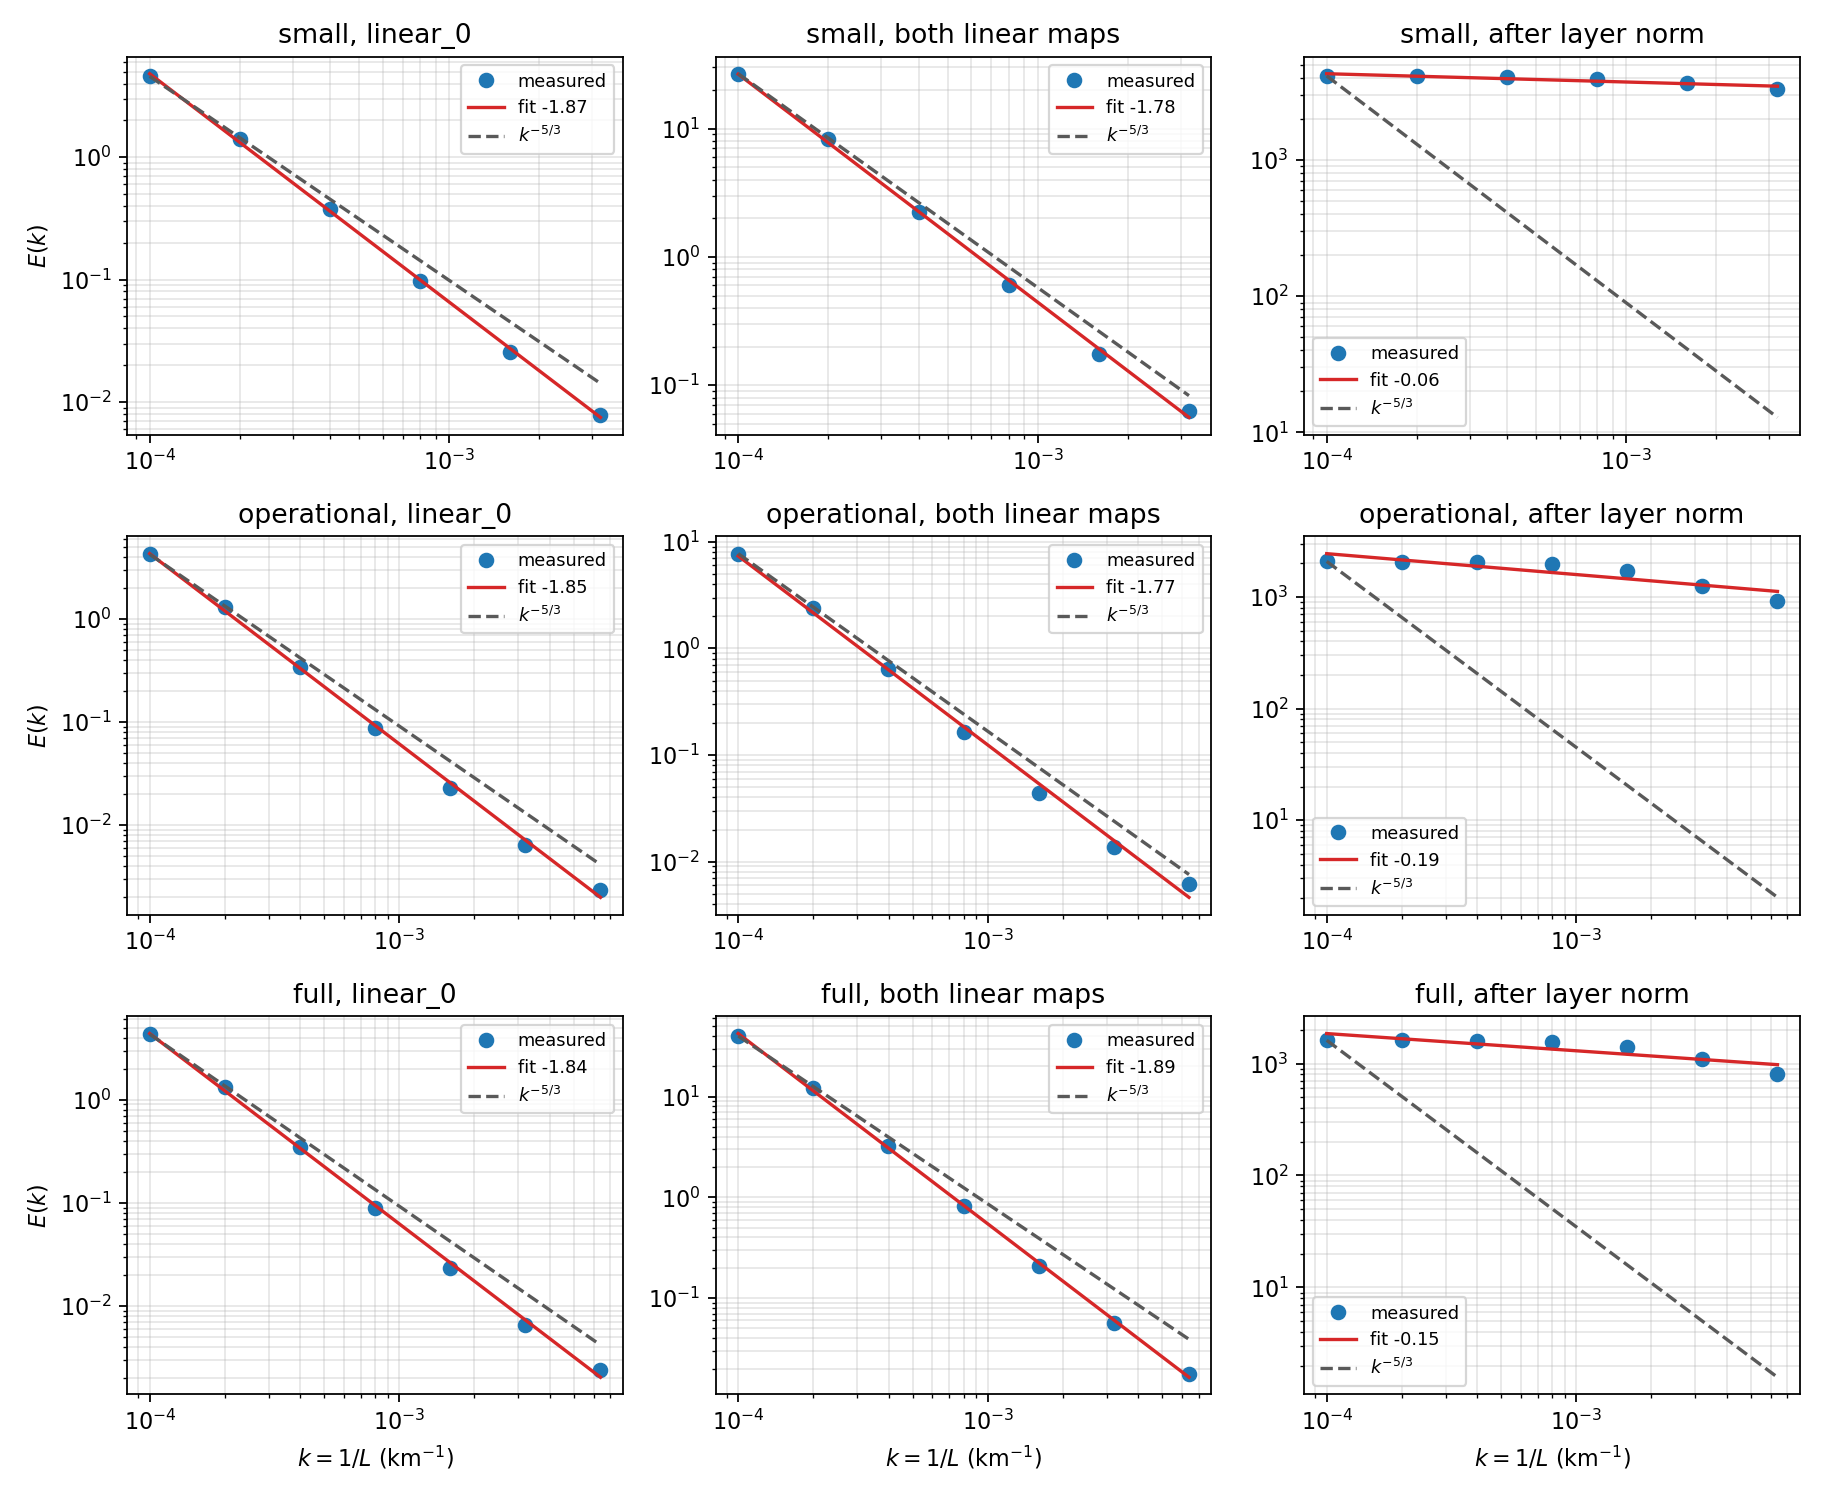
\includegraphics[width=\textwidth]{outputs/graphcast_weight_powerlaw.png}
\caption{Energy against \(k = 1/L\). Each panel is one checkpoint and one stage. Circles are the measured energy. The solid line is the power-law fit of that panel, with its slope in the legend. The dashed line is \(k^{-5/3}\), drawn through that panel's own \(M_0\) energy. Absolute height is not comparable across columns.}
\end{figure}

\section{Why the number changes}

The \(0.835\) nats of the first matrix is fixed by the mesh. A long edge has a larger input than a short one, and \(\|\mathbf{x}\|^2\) scales as length squared. Length halves at each refinement, so \(E(m)\) falls by about a factor of four and the slope sits near \(-2\). The fitted \(-1.87\), with almost all of the variance explained, is that geometric scaling after one linear map. About \(70\%\) of the energy lies on \(M_0\). The small, operational, and full checkpoints agree on this slope and on this share, which is what a shared geometric input should do.

Passing that vector through the second weight matrix does not remove the scaling. Swish is applied to a vector whose size still tracks the edge length, and the second matrix is shared across levels, so the slope only moves from \(-1.87\) to about \(-1.78\) on Small and stays near \(-1.8\) on the other two checkpoints. \(H_n\) stays near \(0.47\) for six levels and near \(0.43\) for seven.

The layer norm is the step that changes the entropy. It divides out the magnitude of each edge, and the magnitude is where the length entered. What remains is the direction of the \(512\)-vector, rescaled by the learned scale and offset. On Small that leaves \(H = 1.789\) nats and \(H_n = 0.998\), with \(17.8\%\) of the energy on \(M_0\) against an equal share of \(16.7\%\). The operational and full checkpoints, which have a seventh level, land at \(H_n = 0.983\) and \(0.987\). The residual slope is shallow, \(-0.06\) on Small and about \(-0.19\) to \(-0.15\) when \(M_6\) is included. That is a property of these weights on the lengths they actually have. It is a different object from an illustration that places energy on ten lengths down to about \(12\,\mathrm{km}\) and quotes an exponent near \(-1/2\).

\end{document}
